\tikzset{
    xaxe style/.style = {
        arrows={-},
        label={},
    }, 
}


\newcommand{\myNumberLineFgColor}{black}
\newcommand{\myNumberLineBgColor}{white}

% #1 : x
% #2 : y
% #3 : point-name
% #4 : solid or empty
\NewDocumentCommand{\myDot}{mO{0} mm}{
    \tkzDefPoint(#1,#2){#3}
    \ifstrequal{#4}{solid}
        {\tkzDrawPoint[line width=1pt, shape=circle, color=\myNumberLineFgColor, size=6,](#3)}
        {}
    \ifstrequal{#4}{empty}
        {\tkzDrawPoint[line width=1pt, shape=circle, color=\myNumberLineFgColor, size=6, fill=\myNumberLineBgColor, ](#3)}
        {}
}


% #1 : x
% #2 : y
% #3 : point-name
% #4 : solid or empty
% #5 : direction (left or right)
% #6 : length
\NewDocumentCommand{\myDotArrow}{m O{0} mmm O{1}}{
    \tkzDefPoint(#1,#2){#3}
    \makeatletter
        \ifstrequal{#5}{left}{\tkzDefShiftPoint[#3](0:-#6){#3@tip}}{}
        \ifstrequal{#5}{right}{\tkzDefShiftPoint[#3](0:#6){#3@tip}}{}

        \tkzDrawSegment[arrows={-{Straight Barb}}, color=\myNumberLineFgColor, line width=2pt,](#3,#3@tip)
    \makeatother
    \ifstrequal{#4}{solid}
        {\tkzDrawPoint[line width=1pt, shape=circle, color=\myNumberLineFgColor, size=6,](#3)}
        {}
    \ifstrequal{#4}{empty}
        {\tkzDrawPoint[line width=1pt, shape=circle, color=\myNumberLineFgColor, size=6, fill=\myNumberLineBgColor, ](#3)}
        {}
}

% #1 : x1,y1
% #2 : point-name-1
% #3 : solid or empty
%
% #4 : x2,y2
% #5 : point-name-2
% #6 : solid or empty
\NewDocumentCommand{\myBetweenSegment}{mmm mmm}{
    \tkzDefPoint(#1){#2}
    \tkzDefPoint(#4){#5}
    \tkzDrawSegment[arrows={-}, color=\myNumberLineFgColor, line width=2pt,](#2,#5)

    \ifstrequal{#3}{solid}{\tkzDrawPoint[line width=1pt, shape=circle, color=\myNumberLineFgColor, size=6,](#2)}{}
    \ifstrequal{#3}{empty}{\tkzDrawPoint[line width=1pt, shape=circle, color=\myNumberLineFgColor, size=6, fill=\myNumberLineBgColor, ](#2)}{}

    \ifstrequal{#6}{solid}{\tkzDrawPoint[line width=1pt, shape=circle, color=\myNumberLineFgColor, size=6,](#4)}{}
    \ifstrequal{#6}{empty}{\tkzDrawPoint[line width=1pt, shape=circle, color=\myNumberLineFgColor, size=6, fill=\myNumberLineBgColor, ](#4)}{}
}





\begin{tikzpicture}
    \tkzInit[xmax=6,xstep=1]
    \tkzDrawX[left space=1, right space=1, text=blue, color=red, label=$t$,]
    \tkzLabelX[text=blue,below = 3pt]

    \myDot{2}{A}{solid}
    \myDot{4}{B}{empty}
\end{tikzpicture}

\noindent
\begin{tikzpicture}
    \tkzInit[xmax=6,xstep=1]
    \tkzDrawX[left space=1, right space=1, label={},]

    \myDot{2}{A}{empty}
    \myDot{4}{B}{solid}
    \tkzLabelPoint[below=2pt,black](A){$2$}
    \tkzLabelPoint[below=2pt,black](B){$4$}

    \tkzDefPoint(3,0){P-middle}
    \tkzLabelPoint[below=2pt,black](P-middle){{\tiny X}}
\end{tikzpicture}


\noindent
\begin{tikzpicture}
    \tkzInit[xmax=6,xstep=1]
    \tkzDrawX[left space=1, right space=1, label={}, ]

    \myBetweenSegment{2,0}{A}{empty}{4,0}{B}{solid}
\end{tikzpicture}



\noindent
\begin{tikzpicture}
    \tkzInit[xmax=6,xstep=1]
    \tkzDrawX[left space=1, right space=1, label={},]

    \myDotArrow{2}{A}{empty}{left}
    \myDotArrow{4}{A}{empty}{right}
\end{tikzpicture}



\noindent
\begin{tikzpicture}
    \tkzInit[xmax=6,xstep=1]
    \tkzDrawX[left space=1, right space=1, label={},]

    \myDotArrow{1}{A}{empty}{left}
    \myBetweenSegment{2,0}{B}{empty}{4.5,0}{C}{solid}
    \myDotArrow{6}{D}{solid}{right}
\end{tikzpicture}



\noindent
\begin{tikzpicture}
    \tkzInit[xmax=6,xstep=1]
    \tkzDrawX[left space=1, right space=1, label={},]

    \myDotArrow{4}[0.2]{A}{empty}{left}[4]
    \myDotArrow{2}[-0.2]{D}{solid}{right}[4]
\end{tikzpicture}
